% Flow of vector components in a normalizing flow coupling layer. Inspired by Ari Seff in https://youtu.be/i7LjDvsLWCg?t=472.

\documentclass[tikz]{standalone}

\usepackage{mathtools}

\usetikzlibrary{calc,positioning,shapes.geometric}

\renewcommand\vec[1]{\boldsymbol{#1}}

\begin{document}
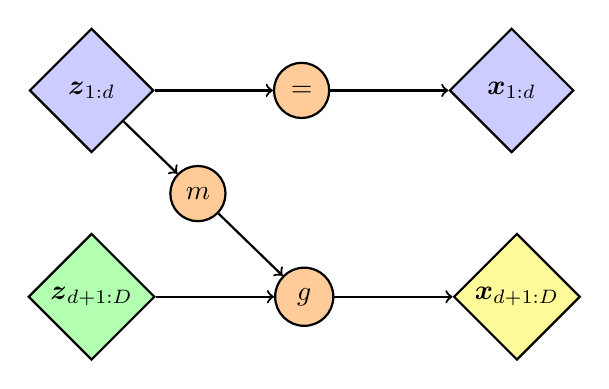
\begin{tikzpicture}[
    thick, node distance=15mm,
    set/.style={draw, diamond, text width=9mm, align=center},
    op/.style={draw, circle, text width=1.em, align=center, fill=orange!40},
  ]

  \node[set, fill=blue!20] (z1) {$\vec z_{1:d}$};
  \node[op, right=of z1] (eq) {\raisebox{-1ex}=};
  \node[set, right=of eq, fill=blue!20] (x1) {$\vec x_{1:d}$};
  \draw[->] (z1) edge (eq) (eq) edge (x1);

  \node[set, below=1 of z1, fill=green!30] (z2) {$\mathclap{\vec z_{d+1:D}}$};
  \node[op, right=of z2] (g) {$g$};
  \node[set, right=of g, fill=yellow!40] (x2) {$\mathclap{\vec x_{d+1:D}}$};
  \draw[->] (z2) edge (g) (g) edge (x2);

  \node[op] (m) at ($(z1)!0.5!(g)$) {$m$};
  \draw[->] (z1) edge (m) (m) edge (g);

\end{tikzpicture}
\end{document}